%# -*- coding: utf-8-unix -*-
%%==================================================
%% chapter_5.tex for SJTU Master Thesis
%%==================================================

\chapter{基于stateflow的PTP时钟同步仿真系统搭建及算法验证}
为了能够对本论文中所提出的优化算法进行验证,本人在实验室师兄的基础上,继续利用stateflow工具,搭建并优化了基于IEEE1588协议的时钟同步系统。为了能够实现仿真验证,该系统中创建了三台ptp时钟,包括两个普通时钟和一个边界时钟,其中一个普通时钟扮演Grand Master的角色,另一个时钟扮演从时钟角色。边界时钟在二者中间,与GM时钟进行同步,同时向从时钟发送Sync报文,最终达到三者处于同步。

下面仅对该仿真系统中比较重要的部分进行介绍,同时利用该系统来进行仿真验证上文所提算法。

\section{仿真系统搭建及介绍}
Simulink Stateflow工具箱是matlab平台上的一种可视化建模工具,对于状态机、流程图等的创建,或者对PTP时钟同步系统之类事件驱动系统进行建模仿真具有非常良好的应用性。

\begin{figure}[!hbp]
  \centering
  \begin{minipage}[b]{1\textwidth}
    \captionstyle{\centering}
    \centering
    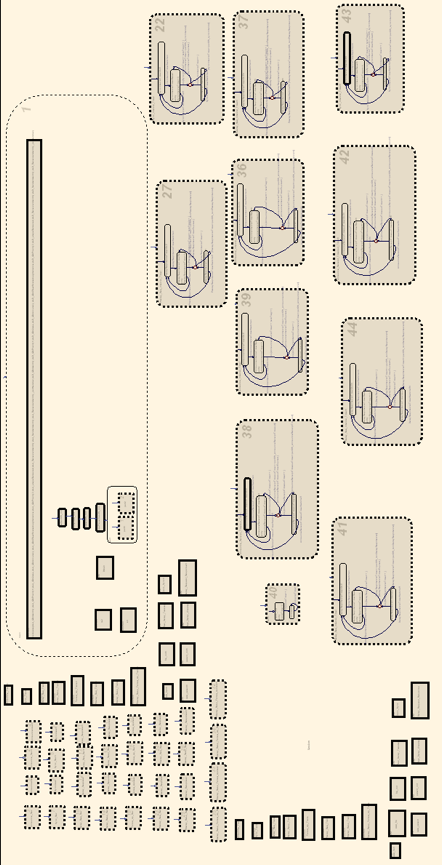
\includegraphics[width=10cm]{simulation_clock_model}
    \bicaption[fig:simulation_clock_model]{基于stateflow的ptp时钟仿真模型}{基于stateflow的ptp时钟仿真模型}{Fig}{The Simulation model of ptp clock based on stateflow}
  \end{minipage}     
\end{figure}

图\ref{fig:simulation_clock_model}中是我们利用stateflow在matlab平台上搭建的单个ptp时钟。该时钟具备两个端口,下面对其中与本文算法相关的一些模块进行简要地介绍,其他模块只给出实现图,不作过多赘述。

\subsection{本地时钟模块}
本地时钟模块:该模块为时钟模块提供本地时钟,对同步系统而言,我们就是要让从时钟的本地时钟模块能够在算法校正后实现与主时钟本地时钟模块保持一致,才算达到良好的同步效果。在实际系统中为晶振驱动,在我们的仿真模型中,使用脉冲生成器来驱动,在每个脉冲上升沿处使的脉冲计数器加pulseCount值,另外设rate值来调节本地时钟精度。例如,使用的脉冲器为100MHz,那么脉冲计数器pulseCount每次累加10ns,如果我们用rate=100,那么表示每100个10ns对应1个时钟clock,即1微秒。我们用clockCount来表示本地时钟,每产生一个clock就使clockCount加1。另外,由于真实的时钟还存在频率偏差,为了模仿这种情况,我们再给pulseCount添加一个偏差值,frequncyOffset,即:
\begin{align}
	clockCount = (pulseCount + frequncyOffset) / rate
\end{align}
对于该频率偏差frequncyOffset,我们应该用时钟伺服系统来进行校正。
\begin{figure}[!hbp]
  \centering
  \begin{minipage}[b]{1\textwidth}
    \captionstyle{\centering}
    \centering
    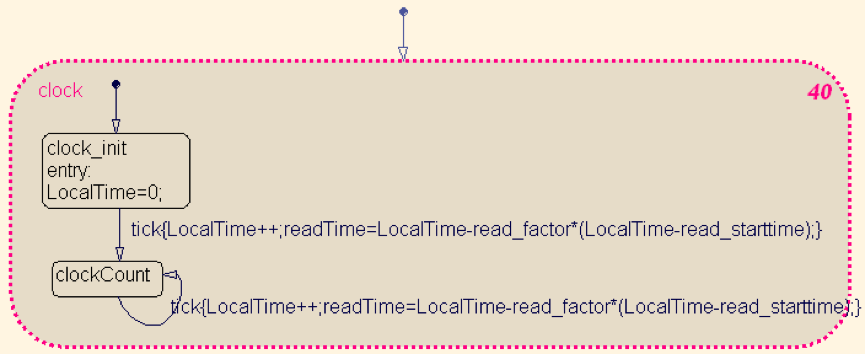
\includegraphics[width=10cm]{simulation_local_clock}
    \bicaption[fig:simulation_local_clock]{本地时钟仿真模型}{本地时钟仿真模型}{Fig}{The Simulation model of Local Clock}
  \end{minipage}     
\end{figure}

\subsection{定时器模块}
由于同步系统中存在很多中定时触发或超时事件,例如Sync报文的周期性发送,Announce报文的超时等待事件等。所以,我们添加了这个模块,为系统中所有周期性或有超时发生的事件进行触发。

下图是Announce超时事件定时器模块作为参考,其他定时器模块与之非常类似。
\begin{figure}[!hbp]
  \centering
  \begin{minipage}[b]{1\textwidth}
    \captionstyle{\centering}
    \centering
    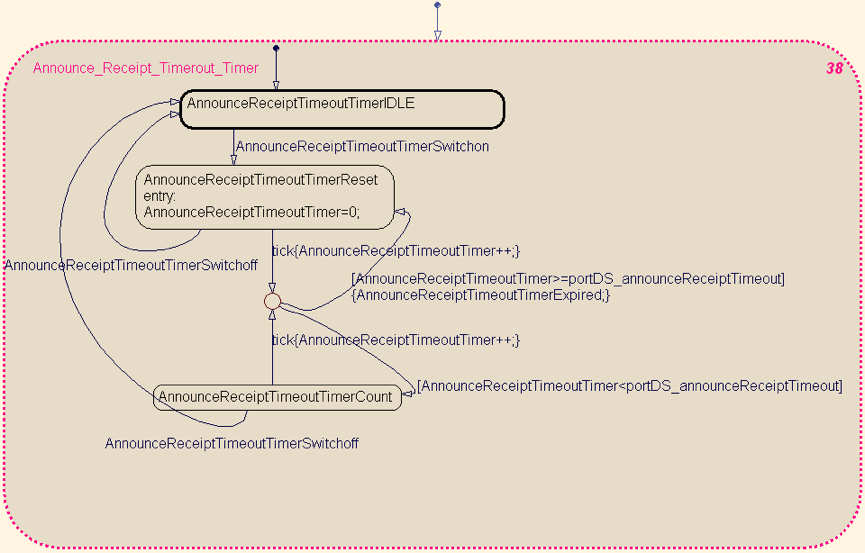
\includegraphics[width=10cm]{simulation_announce_timeout_timer}
    \bicaption[fig:simulation_announce_timeout_timer]{Announce报文超时事件定时器仿真模型}{Announce报文超时事件定时器仿真模型}{Fig}{The Timer model for Announce message receipt timeout}
  \end{minipage}     
\end{figure}

\subsection{最佳主时钟算法及状态机模块}
该模块主要用于根据外部报文数据集来计算并调整本地时钟端口的状态。由于与本文算法关系不大,故不作深入介绍,下为实现图。具体原理可参考上文中的算法介绍。
\begin{figure}[!hbp]
  \centering
  \begin{minipage}[b]{1\textwidth}
    \captionstyle{\centering}
    \centering
    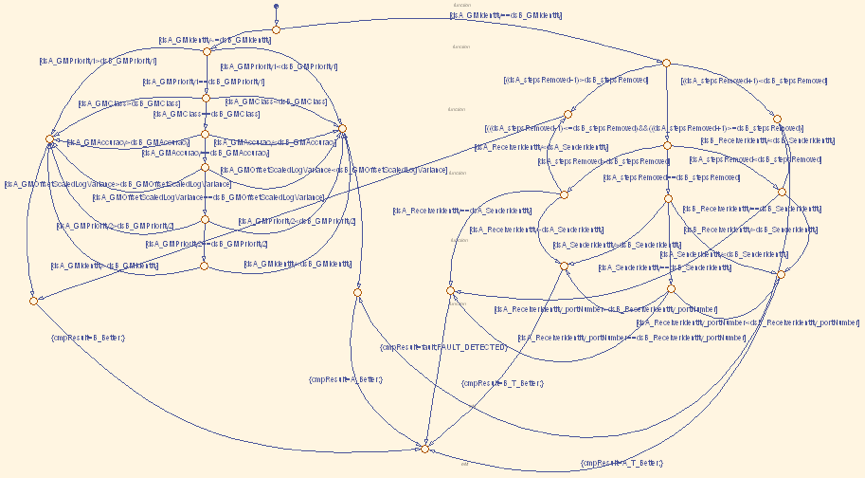
\includegraphics[width=10cm]{simulation_dataset_comparision}
    \bicaption[fig:simulation_dataset_comparision]{数据集比较模块仿真模型}{数据集比较模块仿真模型}{Fig}{The model for dataset comparision}
  \end{minipage}     
\end{figure}

\subsection{报文收发模块}
该模块主要包括每个时钟内部对外的收发报文。对于接收模块,它会时钟监听某外部信号,一旦有报文传入则会立即触发系统进入报文接受流程,该流程会讲所收到报文的数据全部存储到本地,同时向系统中发出报文接受完成信号。对于发送模块,会先把数据根据对应报文格式组装成对应的报文,把数据存入该报文中,然后从时钟对应的端口发出。
\begin{figure}[!hbp]
  \centering
  \begin{minipage}[b]{1\textwidth}
    \captionstyle{\centering}
    \centering
    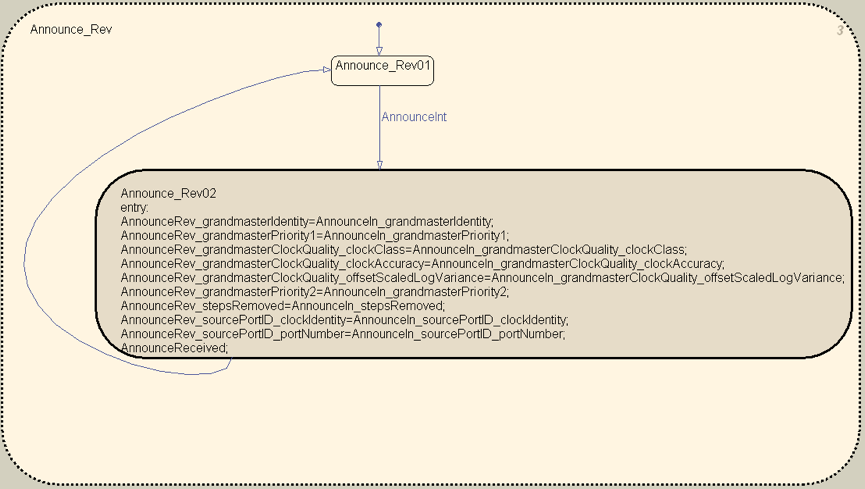
\includegraphics[width=10cm]{simulation_message_receive}
    \bicaption[fig:simulation_message_receive]{报文接收模块仿真模型}{报文接收模块仿真模型}{Fig}{The model for receiving message}
  \end{minipage}     
\end{figure}
\begin{figure}[!hbp]
  \centering
  \begin{minipage}[b]{1\textwidth}
    \captionstyle{\centering}
    \centering
    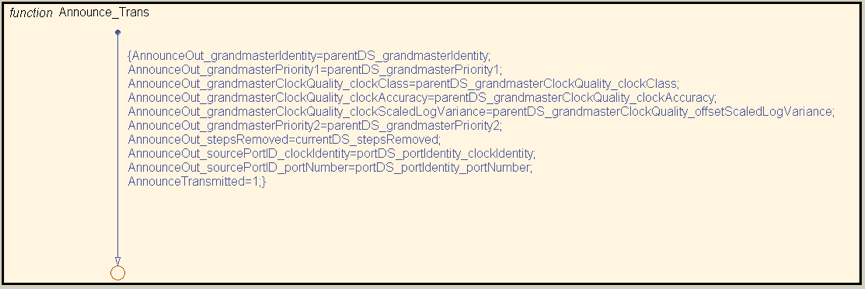
\includegraphics[width=10cm]{simulation_message_send}
    \bicaption[fig:simulation_message_send]{报文发送模块仿真模型}{报文发送模块仿真模型}{Fig}{The model for sending message}
  \end{minipage}     
\end{figure}

\subsection{时钟伺服模块}
这个模块是本节的重点,因为我们的延时统计优化方法和基于神经网络的PID控制策略都是在这个模块中实现的。下面为该模块的外观图,内部主要功能为,获取接受到的链路延时信息,采用统计的方法去计算较为精确的链路延时数据,然后把相关的延时数据传递给神经网络系统中,利用神经网络输出的三个控制参数来对PID控制器进行调解,最后用pid对从时钟本地时钟的相位和频率进行校正。
\begin{figure}[!hbp]
  \centering
  \begin{minipage}[b]{1\textwidth}
    \captionstyle{\centering}
    \centering
    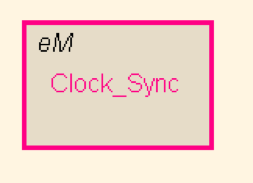
\includegraphics[width=10cm]{simulation_clock_servo_system}
    \bicaption[fig:simulation_clock_servo_system]{时钟伺服模块仿真模型}{时钟伺服模块仿真模型}{Fig}{The model of clock servo system}
  \end{minipage}     
\end{figure}

\section{算法仿真验证思路}
下面,为了验证上述方法的有效性,我们会在自己搭建的1588仿真平台上,分别进行如下验证。
\begin{itemize}[noitemsep,topsep=0pt,parsep=0pt,partopsep=0pt]
  \item 对于传输延时抖动,我们可以在传输中添加随机延时噪声来进行验证;
  \item 对于暂时性时延突变,我们可以对传输延时添加阶跃噪声,并观察对同步过程的影响;
  \item 对于持久性变化,我们可以在运行时链路传输中添加永久性固有延时,并观察结果;
  \item 对于控制策略,我们可以分别采取PI控制器校正和基于神经网络PID控制策略进行同步效果对比。
\end{itemize}

\section{验证指标分析}
在上面本人将所搭建的完整的仿真系统进行了简明扼要的介绍。为了验证本文所提的优化算法,本人会在整个同步系统外部,我们会通过监听主时钟和从时钟的时钟偏差曲线,从而可以知道该同步系统的同步性能。主要的比较指标有下面几点:
\begin{itemize}[noitemsep,topsep=0pt,parsep=0pt,partopsep=0pt]
	\item 偏差值:通过观察主从时钟的偏差值,可以看出该同步系统的同步效果,这也能直接反映真实的同步精度。因此,我们可以以此来检测同步系统中链路延时抖动和“暂时性”抖动对同步精度造成的影响。
	\item 鲁棒性:当系统中发生“持久性”时延变化,那么会造成从时钟发生较大的抖动,所以,我们可以依据此来检测针对“持久性”时延变化的优化算法的效果,如果该优化算法能够使的从时钟的抖动减小,那么表示从时钟的鲁棒性得到了提高。
	\item 收敛速度及稳定性:我们可以通过观察主从偏差的波动值,并计算其收敛时间。尤其是在链路环境发生变化,即类似工业环境中的多种复杂因素导致系统不稳定,以此来观察系统的收敛速度和最终的稳定性,从而来判断本文提出的基于神经网络的PID控制器的效果。
\end{itemize}

\section{对链路时延的数学统计算法的验证}
为了验证上文中提到的“最小二乘线性回归算法”,“动态阈值法”和“实时动态监控算法”的实际效果,下面一次对这三种算法进行验证。在验证中,我们可以通过认为模拟延时抖动、排队堵塞和拓扑结构变化等因素导致的时延变化,通过比较采用相关算法前后的同步曲线来得出相关结论。

下文中的同步曲线是指从时钟与主时钟之间的随时间变化的实时同步偏差曲线。

\subsection{验证“最小二乘线性回归算法”对延时抖动的优化}
为了验证“最小二乘线性回归算法”对延时抖动的优化效果,本人在从时钟计算链路传输延时时添加随机扰动,并模拟该扰动符合标准正态分布,得到下面两个仿真结果。见对比图\ref{fig:添加正态分布随机抖动,且利用“最小二乘线性回归算法”处理前后的同步曲线}。
\begin{itemize}[noitemsep,topsep=0pt,parsep=0pt,partopsep=0pt]
  \item 含有服从正态分布的随机噪声,无任何优化的同步曲线
  \item 含有服从正态分布的随机噪声,利用“最小二乘线性回归算法”优化后的同步曲线
\end{itemize}

\begin{figure}
  \centering
  \subfigure[含有服从正态分布的随机噪声,无任何优化的同步曲线]{
    \label{fig:含有服从正态分布的随机噪声,无任何优化的同步曲线} %% label for first subfigure
    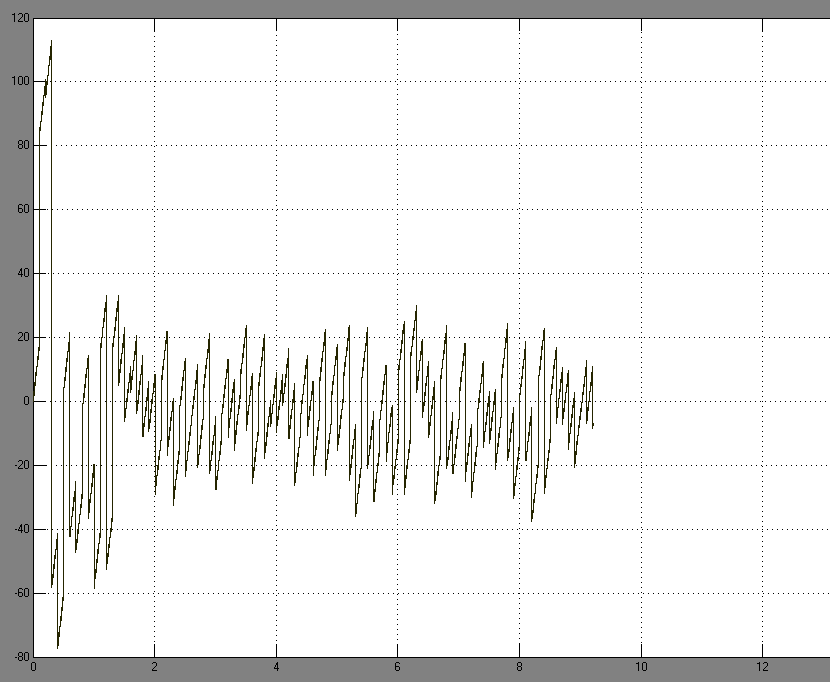
\includegraphics[width=0.6\textwidth]{matlab/添加正态分布的随机抖动后的同步曲线.PNG}}
  \hspace{1in}
  \subfigure[添加正态分布随机抖动且利用最小二乘处理后的同步曲线]{
    \label{fig:添加正态分布随机抖动且利用最小二乘处理后的同步曲线} %% label for second subfigure
    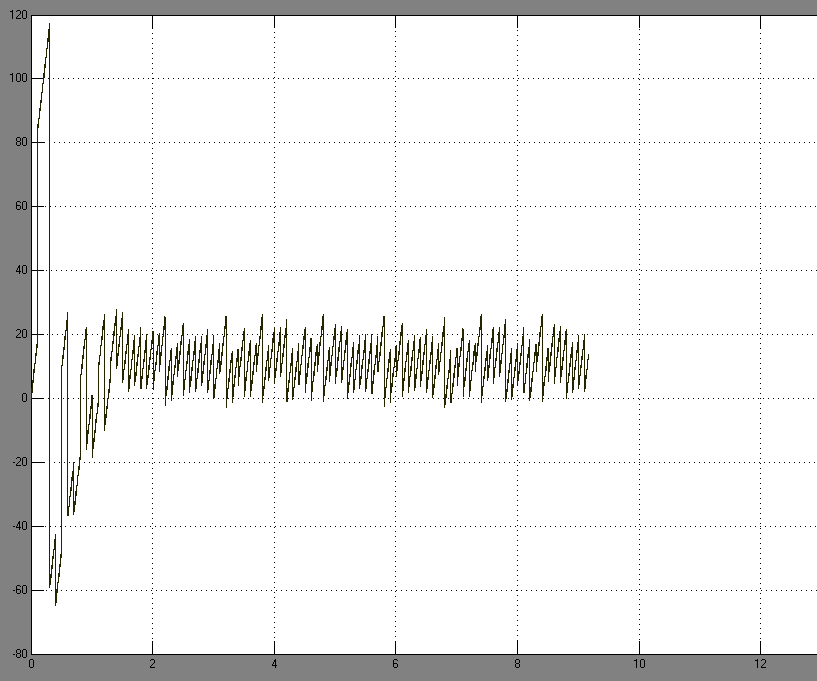
\includegraphics[width=0.6\textwidth]{matlab/添加正态分布随机抖动且利用最小二乘处理后的同步曲线.PNG}}
  \bicaption[fig:添加正态分布随机抖动,且利用“最小二乘线性回归算法”处理前后的同步曲线]{添加正态分布随机抖动,且利用“最小二乘线性回归算法”处理前后的同步曲线}{添加正态分布随机抖动,且利用“最小二乘线性回归算法”处理前后的同步曲线}{Fig}{The Synchronization curve dealing with least square method, within Normal Distribution random noise}
\end{figure}

通过上面的对比曲线,我们可以明显看出,利用最小二乘法处理后可以明显减小随机噪声对同步结果的影响,从时钟振动幅度减小,从时钟具有更好的同步效果。说明该线性回归算法能够很好的减小随机抖动对从时钟系统的影响。

\subsection{验证“动态阈值法”对“暂时性”时延突变的优化}
为了模拟“暂时性”时延变化,我们在同步系统运行中间,突然加入一个时延突变,并保持一小段时间。并分别仿真出采用“动态阈值法”前后的时钟同步曲线。见对比图\ref{fig:添加暂时性时延突变后,采用“动态阈值法”处理前后的同步曲线}。
\begin{itemize}[noitemsep,topsep=0pt,parsep=0pt,partopsep=0pt]
  \item 在接近2秒时,添加暂时性时延突变,无任何优化的同步曲线
  \item 在接近2秒时,添加暂时性时延突变,利用“动态阈值法”优化后的同步曲线
\end{itemize}

\begin{figure}
  \centering
  \subfigure[添加暂时性时延突变后的同步曲线]{
    \label{fig:添加暂时性时延突变后的同步曲线} %% label for first subfigure
    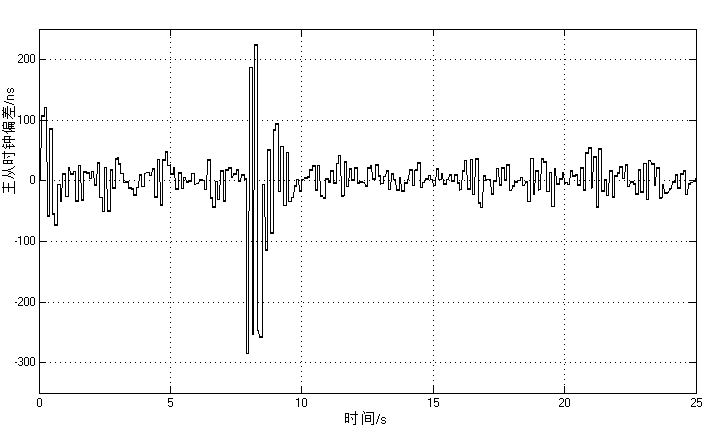
\includegraphics[width=0.6\textwidth]{matlab/添加暂时性时延突变后的同步曲线.PNG}}
  \hspace{1in}
  \subfigure[添加暂时性时延突变并采用动态阈值法处理后的同步曲线]{
    \label{fig:添加暂时性时延突变并采用动态阈值法处理后的同步曲线} %% label for second subfigure
    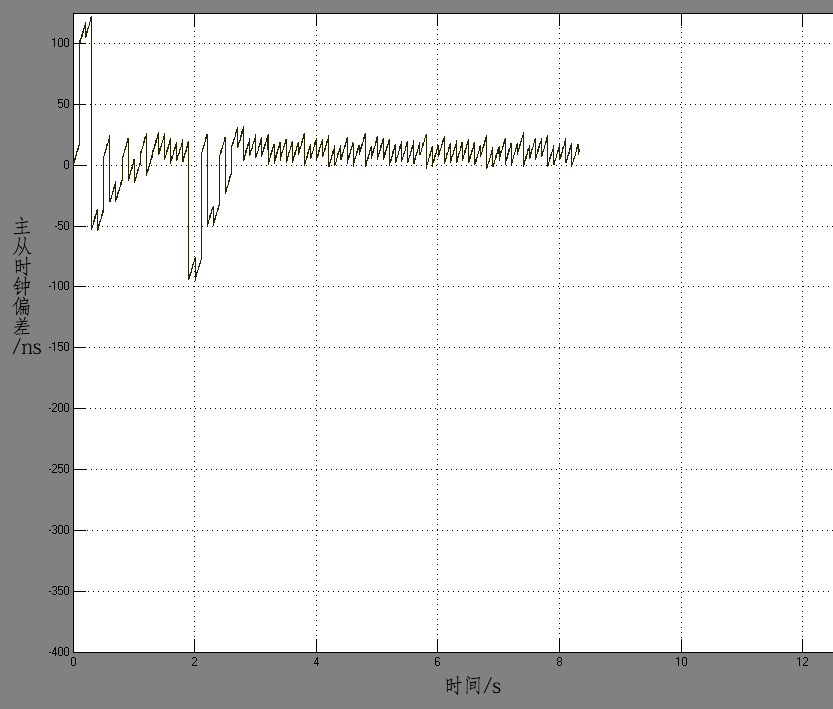
\includegraphics[width=0.6\textwidth]{matlab/添加暂时性时延突变并采用动态阈值法处理后的同步曲线.PNG}}
  \bicaption[fig:添加暂时性时延突变后,采用“动态阈值法”处理前后的同步曲线]{添加暂时性时延突变后,采用“动态阈值法”处理前后的同步曲线}{添加暂时性时延突变后,采用“动态阈值法”处理前后的同步曲线}{Fig}{The Synchronization curve dealing with dynamic threshold value method, within temporary time-delay mutation}
\end{figure}

通过上面的对比曲线,我们可以明显看出,利用了“动态阈值法”对阶跃噪声进行优化后,从时钟的瞬间振荡明显减小,这意味着从时钟具备了更好的鲁棒性和稳定性,不会轻易随着网络负载变化而发生较大波动。

\subsection{验证“实时动态监控算法”对“持久性”时延变化的优化}
为了模拟“持久性”时延变化,我们在同步系统运行中间,加入一个恒定的时延变化,并保持不变。然后分别仿真出采用“实时动态监控算法”前后的时钟同步曲线。见对比图\ref{fig:添加持久性时延突变后,采用“实时动态监控算法”处理前后的同步曲线}。
\begin{itemize}[noitemsep,topsep=0pt,parsep=0pt,partopsep=0pt]
  \item 在接近2秒时,添加持久性固定延时,无任何优化的同步曲线
  \item 在接近2秒时,添加持久性固定延时,利用“实时动态监控算法”优化后的同步曲线
\end{itemize}
\begin{figure}
  \centering
  \subfigure[添加持久性时延变化后样本逐步覆盖的同步曲线]{
    \label{fig:添加持久性时延变化后样本逐步覆盖的同步曲线} %% label for first subfigure
    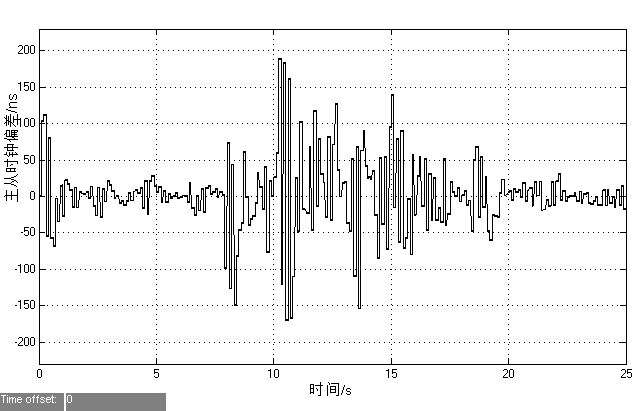
\includegraphics[width=0.6\textwidth]{matlab/添加持久性时延变化后样本逐步覆盖的同步曲线.PNG}}
  \hspace{1in}
  \subfigure[添加持久性时延变化后实时监控处理后的同步曲线]{
    \label{fig:添加持久性时延变化后实时监控处理后的同步曲线} %% label for second subfigure
    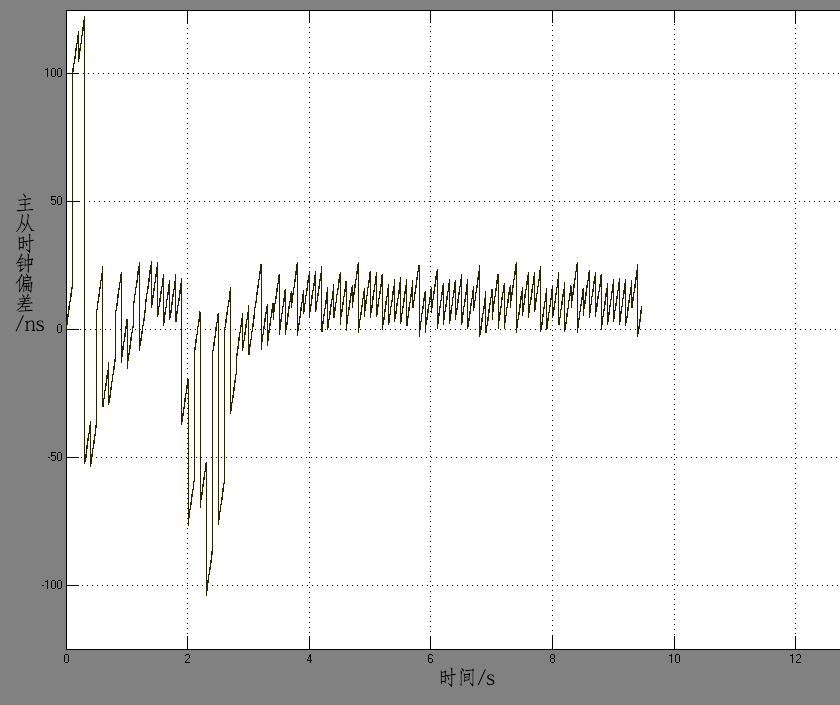
\includegraphics[width=0.6\textwidth]{matlab/添加持久性时延变化后实时监控处理后的同步曲线.PNG}}
  \bicaption[fig:添加持久性时延突变后,采用“实时动态监控算法”处理前后的同步曲线]{添加持久性时延突变后,采用“实时动态监控算法”处理前后的同步曲线}{添加持久性时延突变后,采用“实时动态监控算法”处理前后的同步曲线}{Fig}{The Synchronization curve dealing with real-time dynamic monitoring method, within persistence time-delay change}
\end{figure}

可以发现,利用“实时动态监控算法”对“持久性”时延变化进行实时监控后,可以在系统中发生“持久性”时延变化后通过实时监控能够迅速发现该变化,然后采取相关措施后使得同步过程快速恢复正常,这提高了同步系统对外界变化的快速响应性。

\section{对基于神经网络PID控制算法可行性的验证}
在验证中,我们会随机模拟如时延抖动、排队堵塞等不良网络状况,以此检测算法在实际现场中遭遇到各种随机扰动后同步系统的运行效果。见对比图\ref{fig:添加多种抖动和时延变化后,采用“常规PI控制”与“神经网络PID控制策略”对比的同步曲线}。
\begin{itemize}[noitemsep,topsep=0pt,parsep=0pt,partopsep=0pt]
  \item 采用固定参数的PI控制器校正策略的同步曲线
  \item 采用基于神经网络的PID控制策略的同步曲线
\end{itemize}

\begin{figure}
  \centering
  \subfigure[添加多种抖动和时延变化后的常规PI控制策略同步曲线]{
    \label{fig:添加多种抖动和时延变化后的常规PI控制策略同步曲线} %% label for first subfigure
    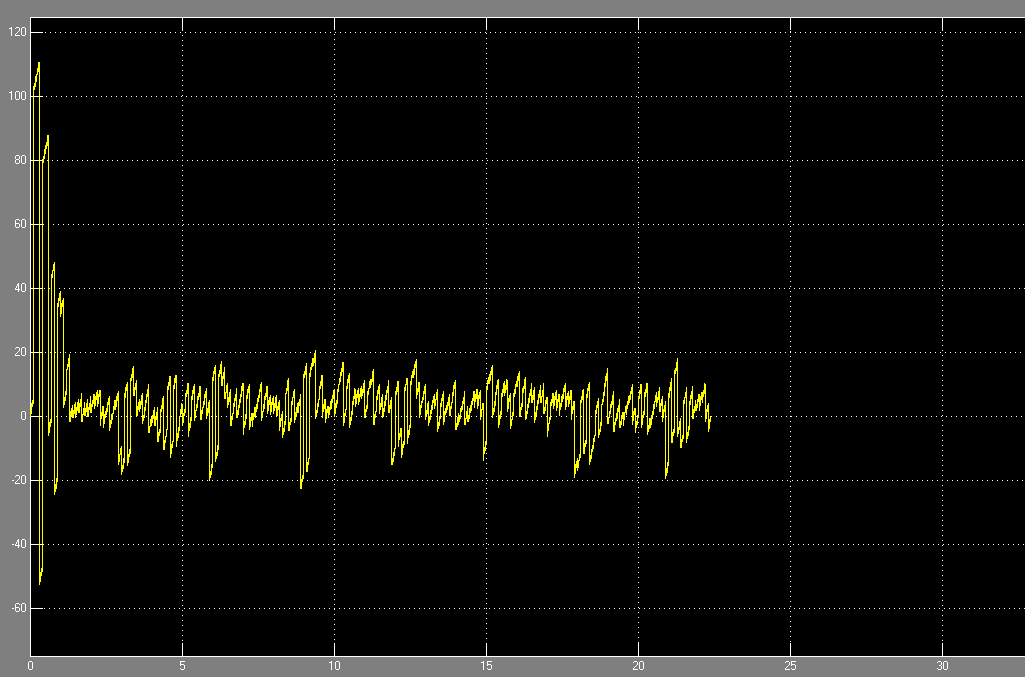
\includegraphics[width=0.6\textwidth]{matlab/添加多种抖动和时延变化后的常规PI控制策略同步曲线.PNG}}
  \hspace{1in}
  \subfigure[添加多种抖动和时延变化后利用神经网络PID处理后的同步曲线]{
    \label{fig:添加多种抖动和时延变化后利用神经网络PID处理后的同步曲线} %% label for second subfigure
    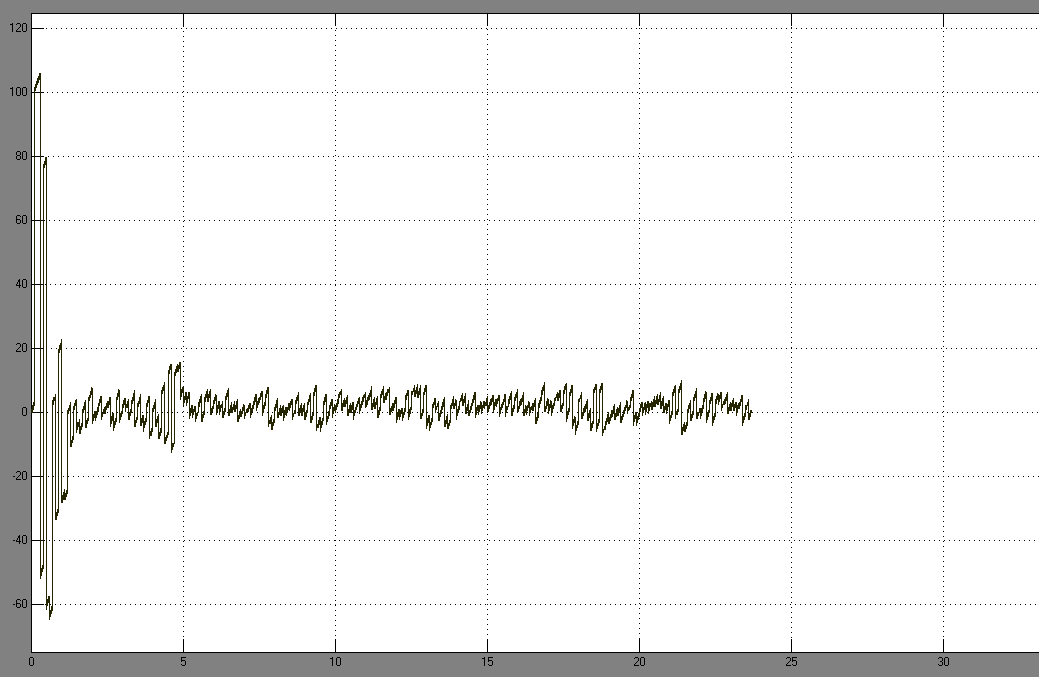
\includegraphics[width=0.6\textwidth]{matlab/添加多种抖动和时延变化后利用神经网络PID处理后的同步曲线.PNG}}
  \bicaption[fig:添加多种抖动和时延变化后,采用“常规PI控制”与“神经网络PID控制策略”对比的同步曲线]{添加多种抖动和时延变化后,采用“常规PI控制”与“神经网络PID控制策略”对比的同步曲线}{添加多种抖动和时延变化后,采用“常规PI控制”与“神经网络PID控制策略”对比的同步曲线}{Fig}{The Synchronization curve dealing with both \"Normal PI Control\" and \"Neural Network PID Control\" method, within kinds of time-delay change}
\end{figure}

通过对比,可以发现PI控制器稳定性较高,具备不错的同步效果,但是一旦系统中发生较为复杂的网络波动,则会发生明显波动,适应性很差。相对而言,采用神经网络的PID控制策略明显具备更好的稳定性和自适应性,它能够实时根据外界环境变化对自身进行调整,从而使的系统能够快速响应外界的变化,从而在实际工业现场有更良好的表现。